\documentclass{article}
\usepackage{parskip}
\usepackage[margin=1.5cm]{geometry}
\usepackage{graphicx}
\usepackage{framed}
\usepackage{float}

\graphicspath{{.}}

% Thanks to Angus Pearson for nagging me to fuck about with fonts in
% XeLaTeX

\usepackage{fontspec} \usepackage{xltxtra}

% PT Serif
\setromanfont[ BoldFont=PTF75F.ttf, ItalicFont=PTZ56F.ttf,
BoldItalicFont=PTF76F.ttf, ]{PTF55F.ttf}

% Noto Sans
\setsansfont[ BoldFont=NotoSans-Bold.ttf,
ItalicFont=NotoSans-Italic.ttf, BoldItalicFont=NotoSans-BoldItalic.ttf
]{NotoSans-Regular.ttf}

\begin{document}

\textbf{\Huge Operating Systems Notes}

\section{OSs and Architectures}

Different architectures dictates the way that an operating system must conduct its business.

As different architecture platforms have different instruction sets, it determines what are viable methods for accomplishing tasks such as \textit{memory protection} and \textit{control interrupts}.

The OS acts as an intermediary between software and hardware. It allows to mediate access and gives developers a nicer way of completing lower-level actions. This abstraction is achieved via \textit{traps} and \textit{exceptions}. Similarly, devices can gain attention via the use of \textit{interrupts}.

An OS is intended to be a good balance between \textit{user needs} and \textit{system needs}.

A user wants an OS to be \textit{fast, reliable and safe}; an OS developer wants it to be \textit{efficient, error-free, and easy to maintain and implement}.

The design of an operating systems makes a distinction between two underlying principles:

\textbf{Policy}, which is \textit{what} will be done; \textbf{Mechanism}, which his \textit{how} to do it.

\subsection{Structure of an OS}

A capable operating system is home to a multitude of components: memory management, I/O, file systems, command interpreters and so on. There are multiple ways to link to structure how all these components are connected to each other.

\subsubsection{Monolithic}

An early type of design for an OS, where the \textit{entire} operating system would function in \textit{kernel mode} (see the \textit{Privileged Instructions} section). However, this design carried many issues with maintainability and reliability, and was hard to make sense of.

\subsubsection{Layering}

As opposed to monolithic, this method implemented the OS as a \textit{set of layers} instead, where a layer could present itself to the corresponding layer above.

\begin{figure}[H]
  \centering
  \begin{center}
  \begin{tabular}{|c|c|l|}
    \hline
    5 & \textbf{Job Managers} & Execute a user's programs\\
    \hline
    4 & \textbf{Device Managers} & Handle devices, provide buffering\\
    \hline
    3 & \textbf{Console Manager} & Provide virtual consoles\\
    \hline
    2 & \textbf{Page Manager} & Implement virtual memories for each process\\
    \hline
    1 & \textbf{Kernel} & Implement a virtual processor for each process\\
    \hline
    0 & \textbf{Hardware} & \\
    \hline
  \end{tabular}
\end{center}
\caption{Dijkstra's THE System}
\end{figure}

\filbreak
\subsection{Privileged Instructions}

These instructions are restricted to use by the OS \textit{only}, and includes direct access to \textit{I/O devices} and \textit{memory state management}.

This is achieved by the implementation of two \textit{modes of operation}; \textit{user} and \textit{kernel} modes.

Privileged instructions can only be executed in kernel mode.

\begin{figure}[h!]
  \centering
  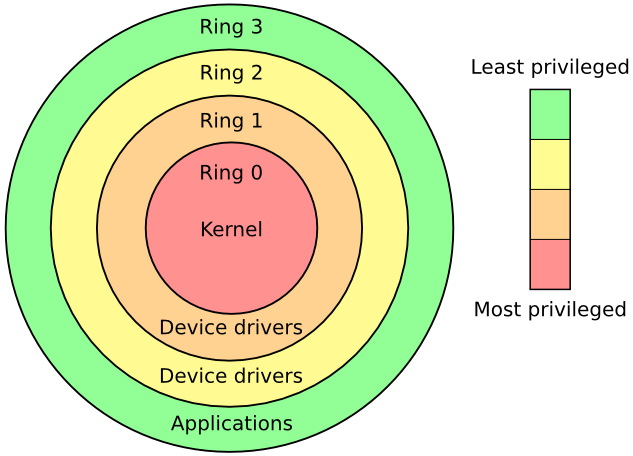
\includegraphics[scale=0.35]{privilegeGraphX86}
  \caption{x86 Architecture Levels of Privilege}
  \textit{\footnotesize Courtesy of Hertzsprung of English Wikipedia}
\end{figure}

\subsubsection{System Calls}

If code running from within user mode tries to execute a privileged instruction, it will trigger the \textit{illegal execution trap}, which allows for such code to gain access to privileged instructions and resources. These are called \textit{system calls}.

An OS will define a set of system calls that makes it possible for such an interaction to take place.

\begin{figure}[H]
  \begin{framed}
    \textit{Caller}: The user mode process invoking the system call\\
    \textit{Callee}: The OS handling the system code\\
    \begin{itemize}
    \item The caller places arguments, especially the \textit{type} of system call, in a specified location
    \item The callee saves the caller's state
    \item The callee verifies the arguments
    \item If valid, the code is run
    \item When the system call has been satisfied, the program counter is set to the return address
    \item Execution is returned to user mode
    \end{itemize}
  \end{framed}
  \caption{A rough breakdown of a system call}
\end{figure}

\subsection{Exception Handling}

A \textit{trap} is a synchronised, intended transition that is initiated by the OS.

An \textit{exception} is also synchronised, however it is an \textit{unexpected} problem with some instruction.

An \textit{interrupt} is \textit{a}synchronous on the other hand, and is caused by some external device.

\filbreak
\section{Memory Management}
Programs must be brought from disk into mmemory and then placed into a process.

The CPU can only access data from memory, not disk.

Register access takes at most 1 CPU clock, but Main Memory can take mayn cycles, causing a \emph{Stall}.

\subsection{Base and Limit Registers}
A set of \emph{base} and \emph{limit registers} define the logical adress space. the CPU must chech every
memory access is valid between the base and the limit for that user. Failure causes a trap to the OS monitor

\subsection{Virtual Address Space}
Logical/Virtual addresses are independent of physical memory.

Hardware translates virtual addresses into physical ones.

Logical/Virtual addresses a process can reference is called the address space.

\subsection{Memory Managment Unit (MMU)}
Effectively is a hash function from logical address to physical address.

a MMU prevents the need for swapped out process to be swapped back into the same physical addresses.

Swapping is not typically supported on mobile devices, more likely to to overwite least used data.


\subsection{Partitioning}
Main memory is usually broken up into two partitions; The OS and user process.

Each process is contained within a single contiguous section on memory.

Realocation registers are used to protect users processes from one another and from canging the OS code.

Some old techniques include:
\begin{itemize}
    \item Fixed Partitions - simple but causes fragmentation often
    \item Variable Partitions - no internal fragmentation, but can leave holes in the physical memory
\end{itemize}

Dynamic Storage-Allocation is possible using First-fit, Best-fir and Worst-fit in terms of hole filling.

\end{document}
